\subsection*{Game World and Settings}

\subsubsection*{World Diagram}
\begin{figure}[H]
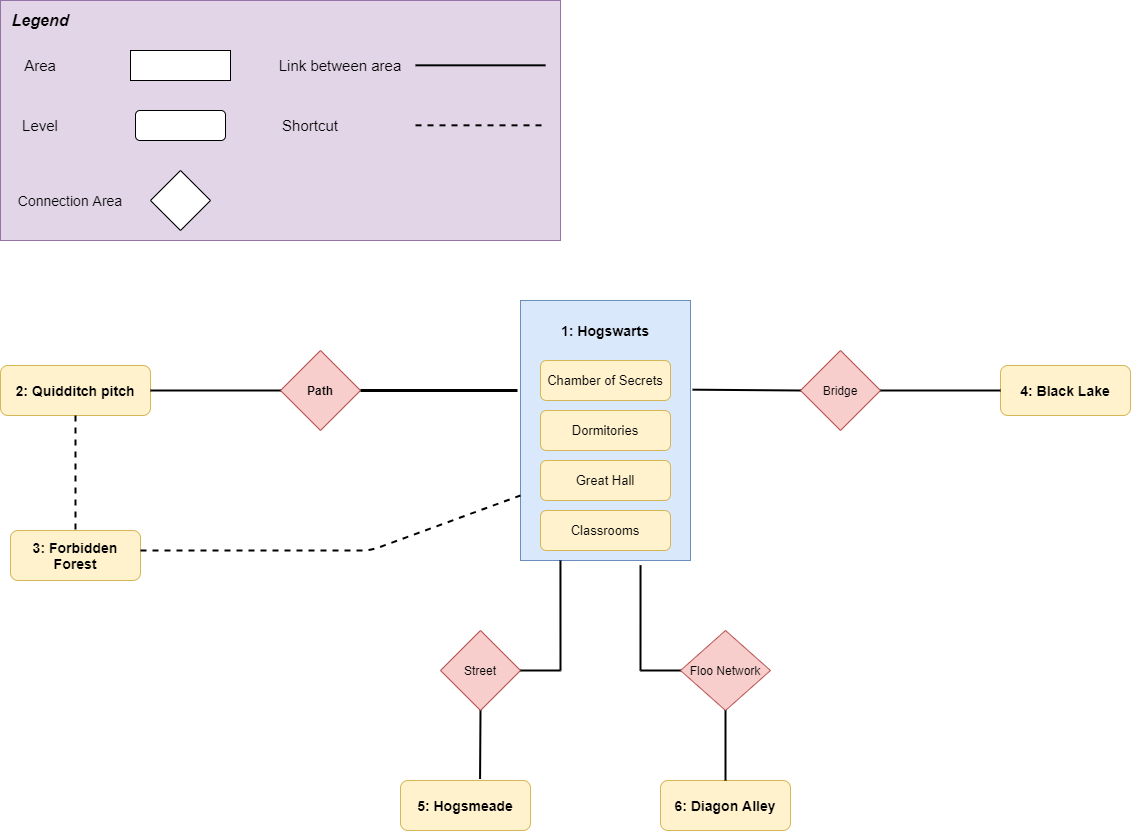
\includegraphics[max width=\textwidth]{../Pictures/Maps/World_diagram.png}
\end{figure}

\subsubsection*{World Maps}
\begin{figure}[H]
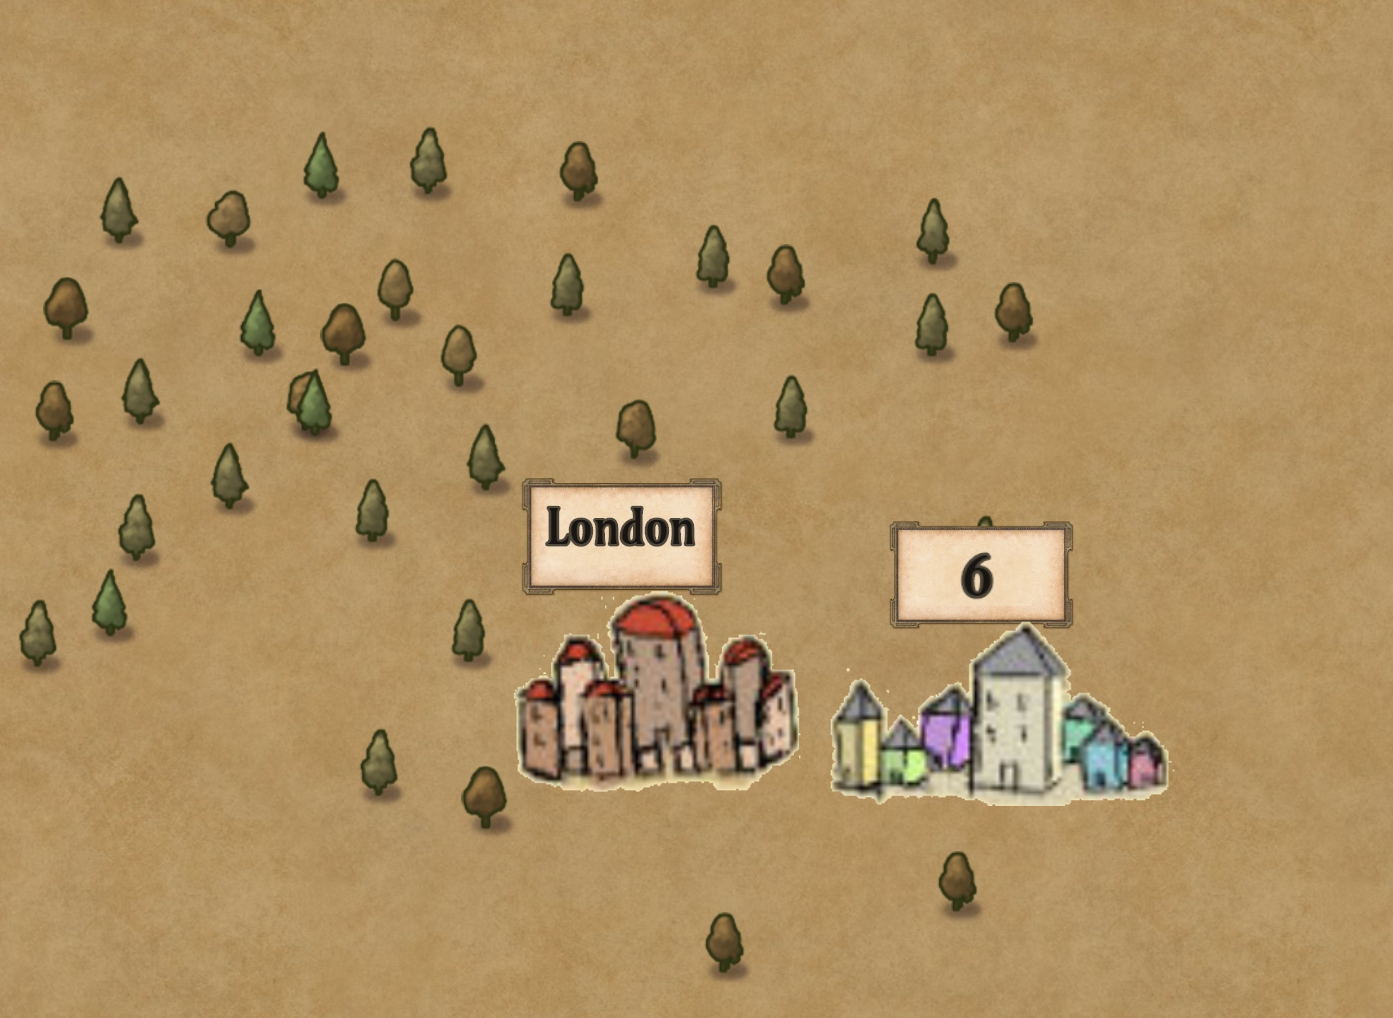
\includegraphics[max width=\textwidth]{../Pictures/Maps/Diagon_Alley_map.png}
\end{figure}
\begin{figure}[H]
\includegraphics[max width=\textwidth]{../Pictures/Maps/Hogwarts_map.png}
\end{figure}

\pagebreak

\subsubsection*{Settings}

\begin{wrapfigure}[14]{r}{0.5\linewidth}
\centering
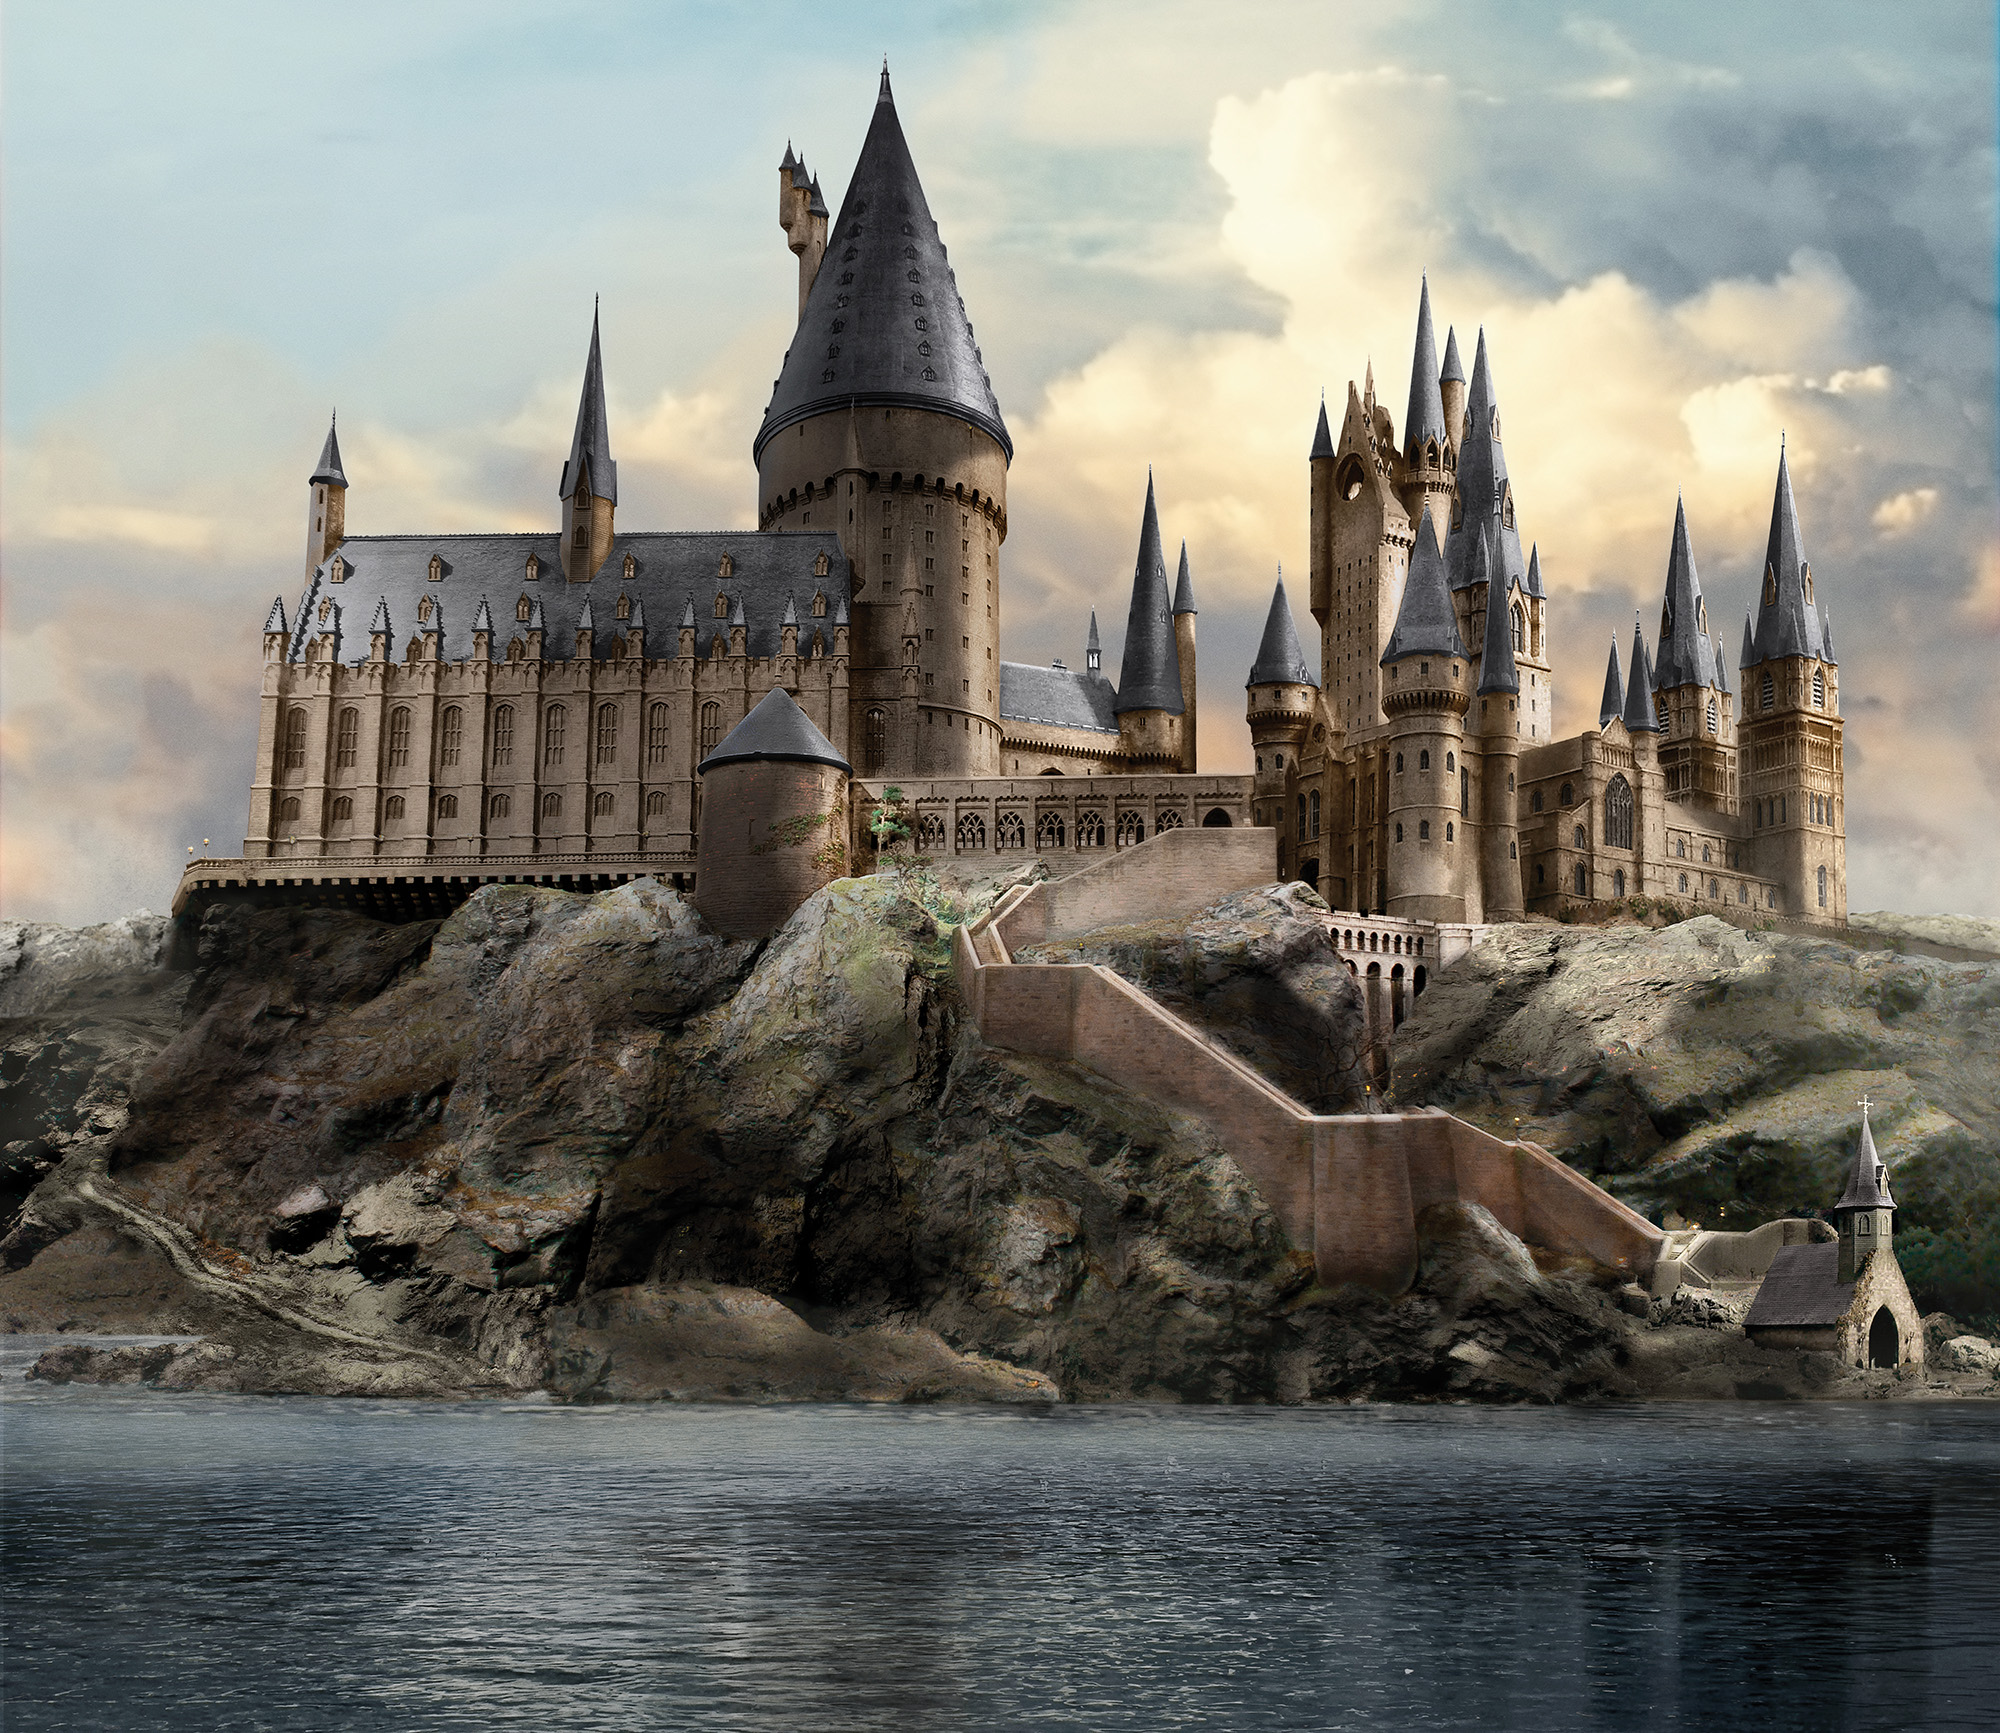
\includegraphics[max width=0.5\textwidth]{../Pictures/Locations/Hogwarts/Castle_picture.png}
\end{wrapfigure}
\paragraph{Hogwarts}
Hogwarts is a School of Witchcraft and Wizardry. It is located in the Highlands Scots, in the United Kingdom. Surrounded by the Black Lake and the Forbidden Forest, the school's castle has its roots at the end of 10th century, which grandeur made it one of the most important schools in the magical world. On the outside, many towers connect the various rooms and halls. In addition, it is surrounded by a green meadow, a Quidditch pitch and other annexed structures, such as the "Keeper of the keys" hut, game and grounds and the green house, where Herbology lessons are held. On the inside, there are seven floors that host classrooms, four dormitories, one Great Hall, and other mysterious rooms. The school has 142 stairways, which each of them seems to have a life of its own as they have fun to change their position and cause poor students to go astray. It is wrapped by many magical protections, making it invisible to muggles: only wizards can live in this castle. 

\paragraph{Great Hall}
The Great Hall is a common place, where all students, the professors, the principal and other staff members of the school gather for the various meals of the day. Furthermore, it acts as a study room, leisure room and ceremonies room. It is composed by four large tables placed vertically, one for each of the houses present in the school, and one large table placed horizontally for the professors and the principal. The Hall is illuminated by thousands of candles that make it cozy and warm for the students. On the ceiling, there is a sky created by a magic spell which mimics the outside. For each recurrence, the hall is embellished, like for Christmas or the Yule Ball. 
\begin{figure}[H]
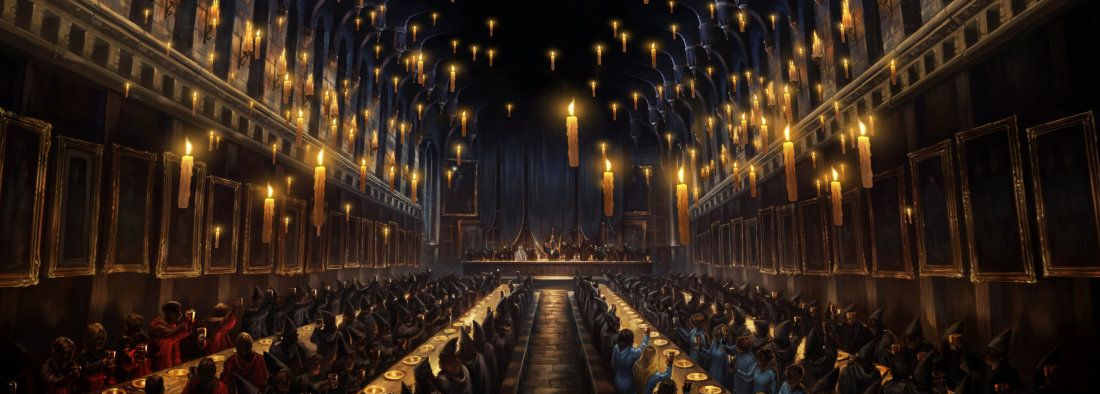
\includegraphics[max width=\textwidth]{../Pictures/Locations/Hogwarts/Great_Hall_picture.jpg} 
\end{figure}

\begin{wrapfigure}[9]{r}{0.5\linewidth}
\centering
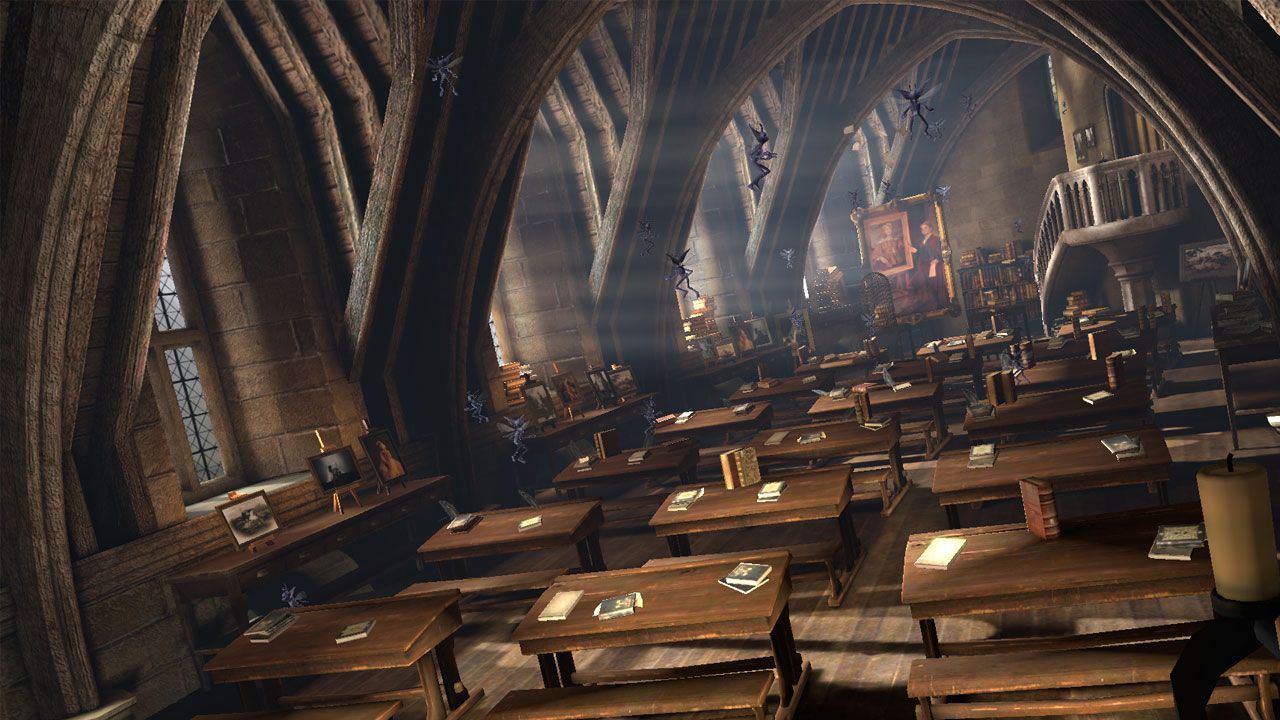
\includegraphics[max width=0.5\textwidth]{../Pictures/Locations/Hogwarts/Classrooms_picture.jpg} 
\end{wrapfigure}
\paragraph{Classrooms}
The classrooms are in various areas of the castle, both inside and outside. The lessons are usually divided into theoretical and practical: the classrooms hosting the practical lessons were embellished according to the topic of the lesson. A great example is Potion-Mixing Room, which has for each bench a cauldron where the student can mix up concoctions and other recipes. The classrooms outside the castle are the Herbology greenhouse and the Quidditch pitch for the Flying Broom lessons. 

\paragraph{Dormitories}
The students are sorted in one of the four Houses present at Hogwarts: Gryffindor, Hufflepuff, Ravenclaw, Slytherin. The Dormitories serve as bedrooms and as a meeting place for students from the same house. Each House is different from the other, in colors and values, and this is represented through decorations and through the students' uniforms.  The dormitories are entrusted to a professor and two prefects (two last year students chosen to enforce the rules within their house). The bedrooms are shared for multiple students with four-poster beds, except for the prefects who have their own private room.
\begin{figure}[H]
\includegraphics[max width=\textwidth]{../Pictures/Locations/Hogwarts/Dorms_picture.png} 
\end{figure}

\begin{wrapfigure}[9]{r}{0.5\linewidth}
\centering
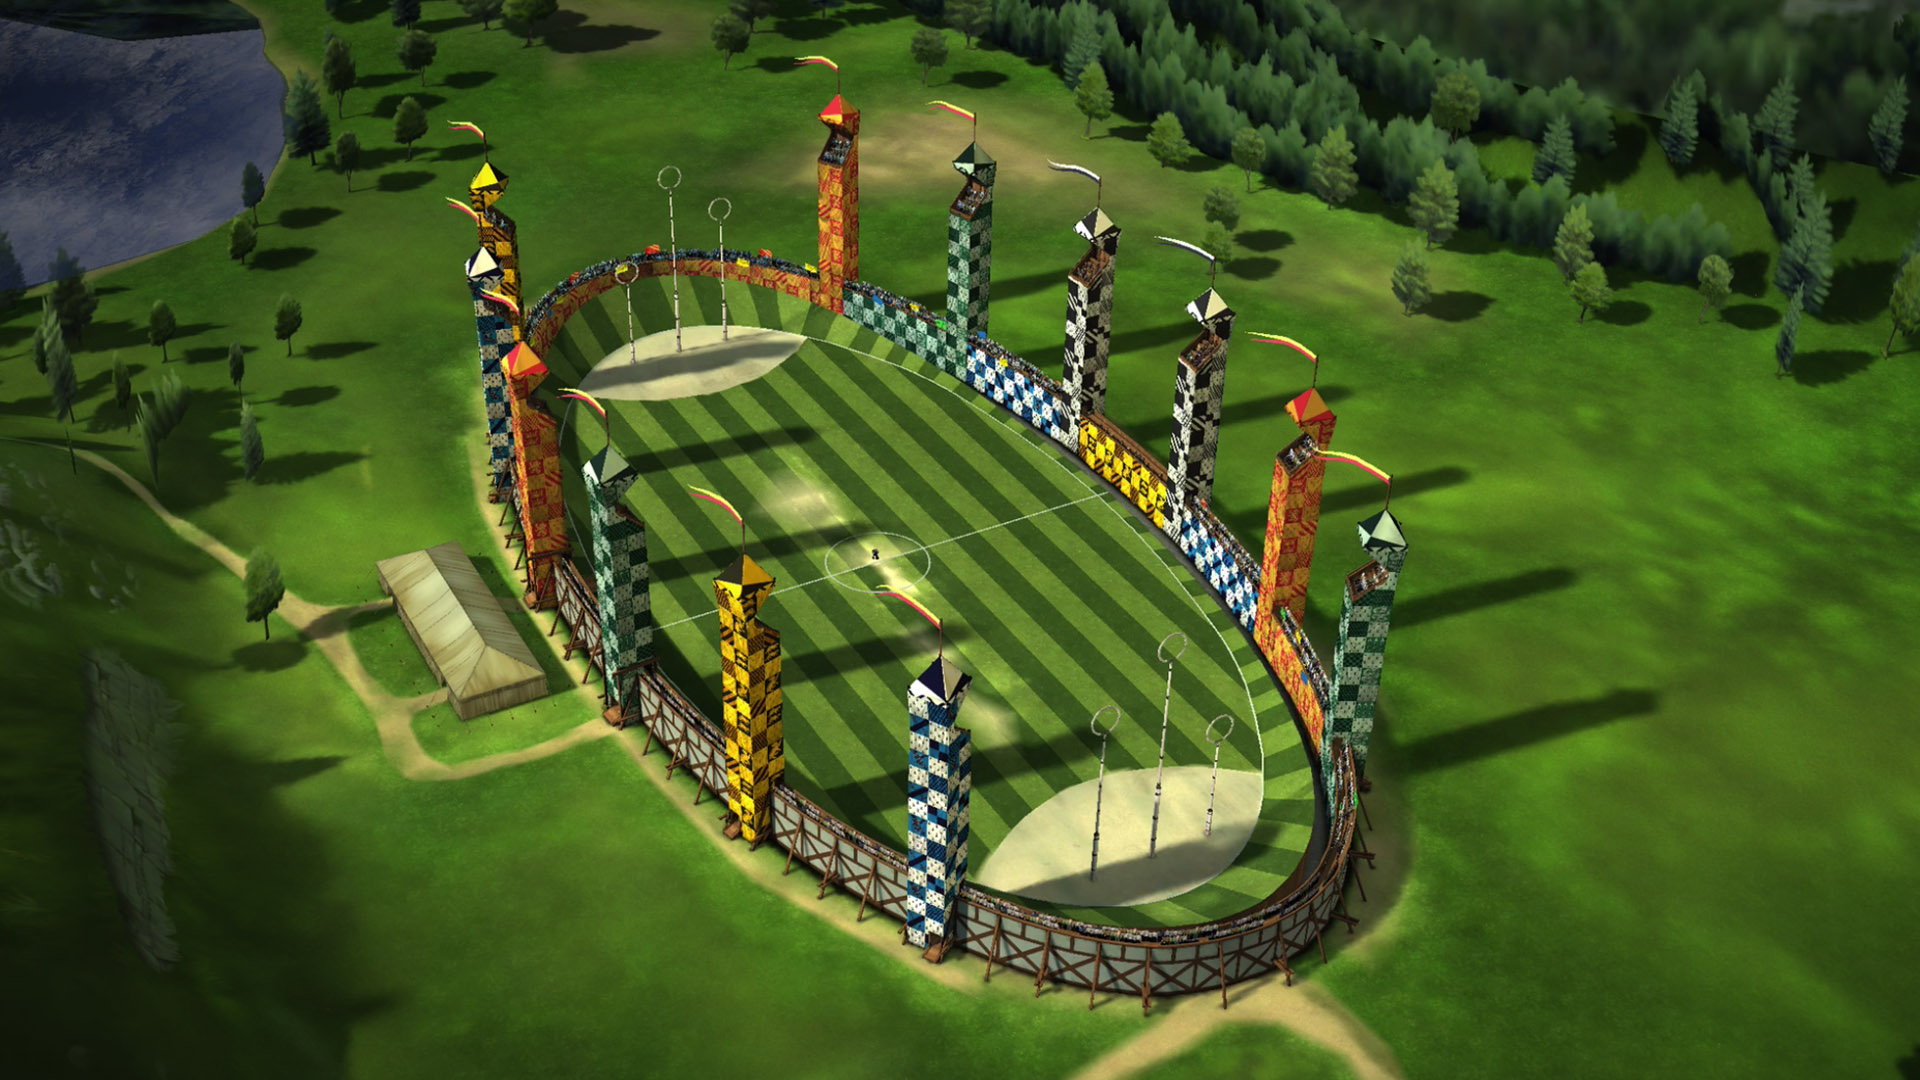
\includegraphics[max width=0.5\textwidth]{../Pictures/Locations/Hogwarts/Quidditch_Field_picture.jpg} 
\end{wrapfigure}
\paragraph{Quidditch pitch}
A huge pitch where students can play Quidditch and train themselves. It is oval in shape and is about 165 meters long by 60 meters wide. At each side there are three goal points of different heights, while below there is a sand area used to soften the falls of the goalkeepers. The surface of the pitch is usually grass, but in some cases, it can be sand or even water. There are several towers for spectators.

\paragraph{Chambers of Secrets}
It's a secret room under the Hogwarts foundation. The entrance is in the girls' bathroom on the second floor and requires saying a secret word in parseltongue for the secret passage to open up. The room is gloomy and dark and has a long corridor where statues in the shape of a snake's head are placed on the sides. In the center stands a colossal statue by Salazar Slytherin, the ancestor and founder of the Slytherin house.  
\begin{figure}[H]
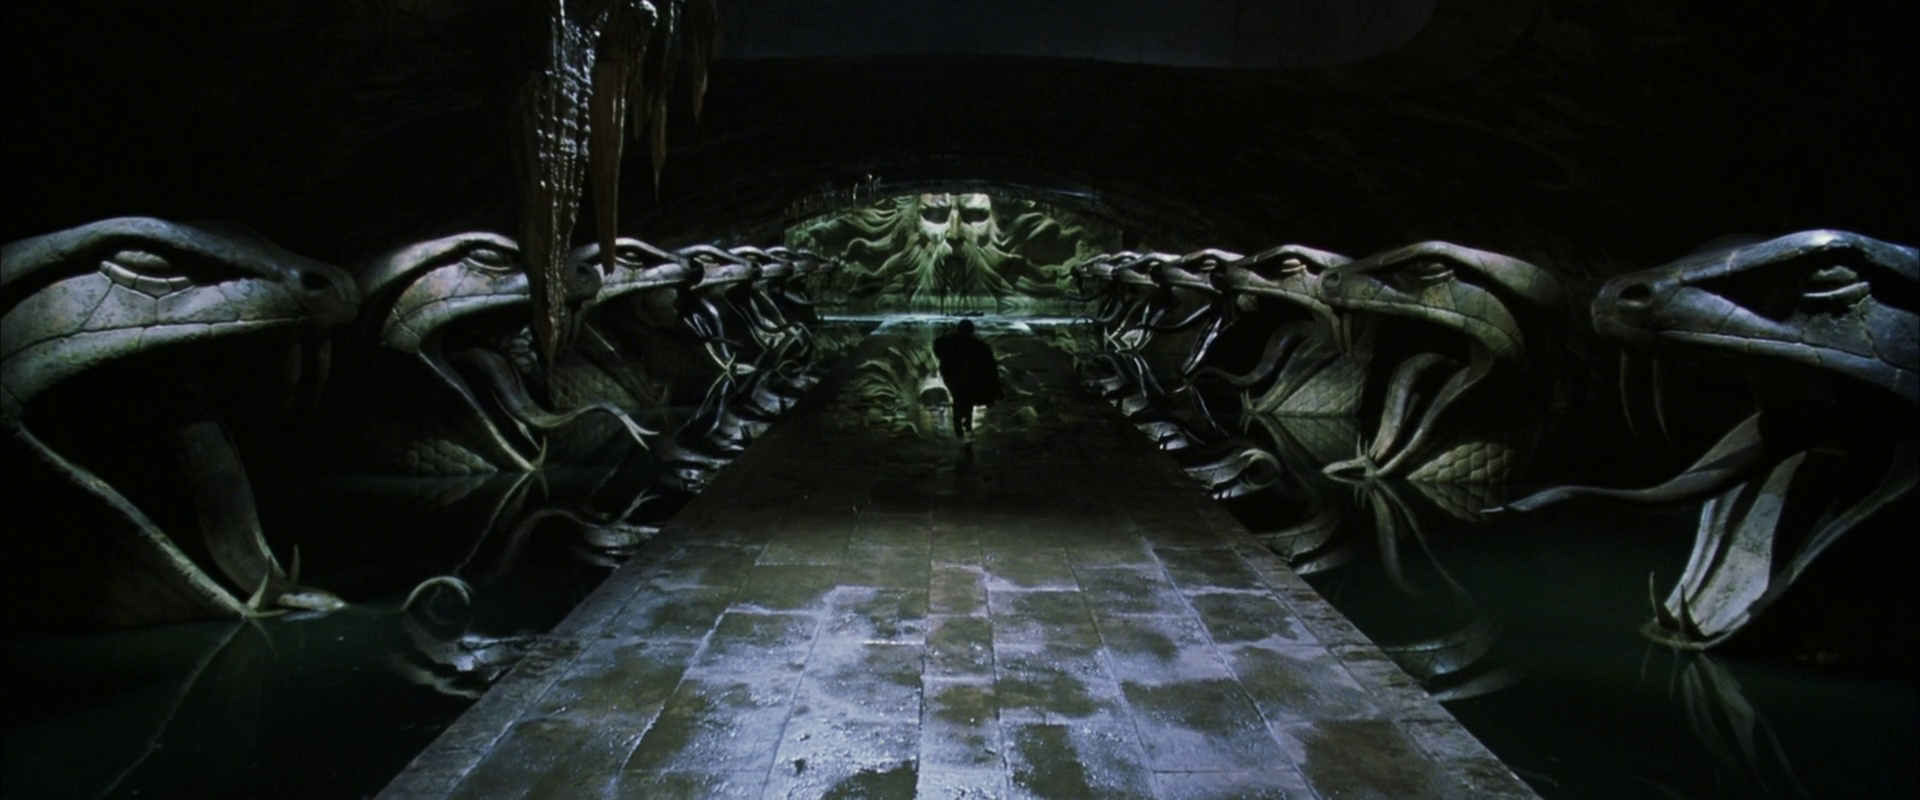
\includegraphics[max width=\textwidth]{../Pictures/Locations/Hogwarts/Chamber_Secrets_picture.png} 
\end{figure}

\paragraph{Forbidden Forest}
It is a large woodland that surrounds part of the castle. It is an area that holds many secret and dangerous wild creatures, such as werewolves, but also beneficial ones, like unicorns. It is also home to many villages, such as the centaur one who take care of the woods. The Forbidden Forest, however, is still considered a place that houses dark entities: as a matter of fact, at night it is impractical to walk in the forest, as if the trees hold inside all the darkness. Even during the day it is very difficult to walk along the path. It is for all these reasons that students are usually denied access to it. 
\begin{figure}[H]
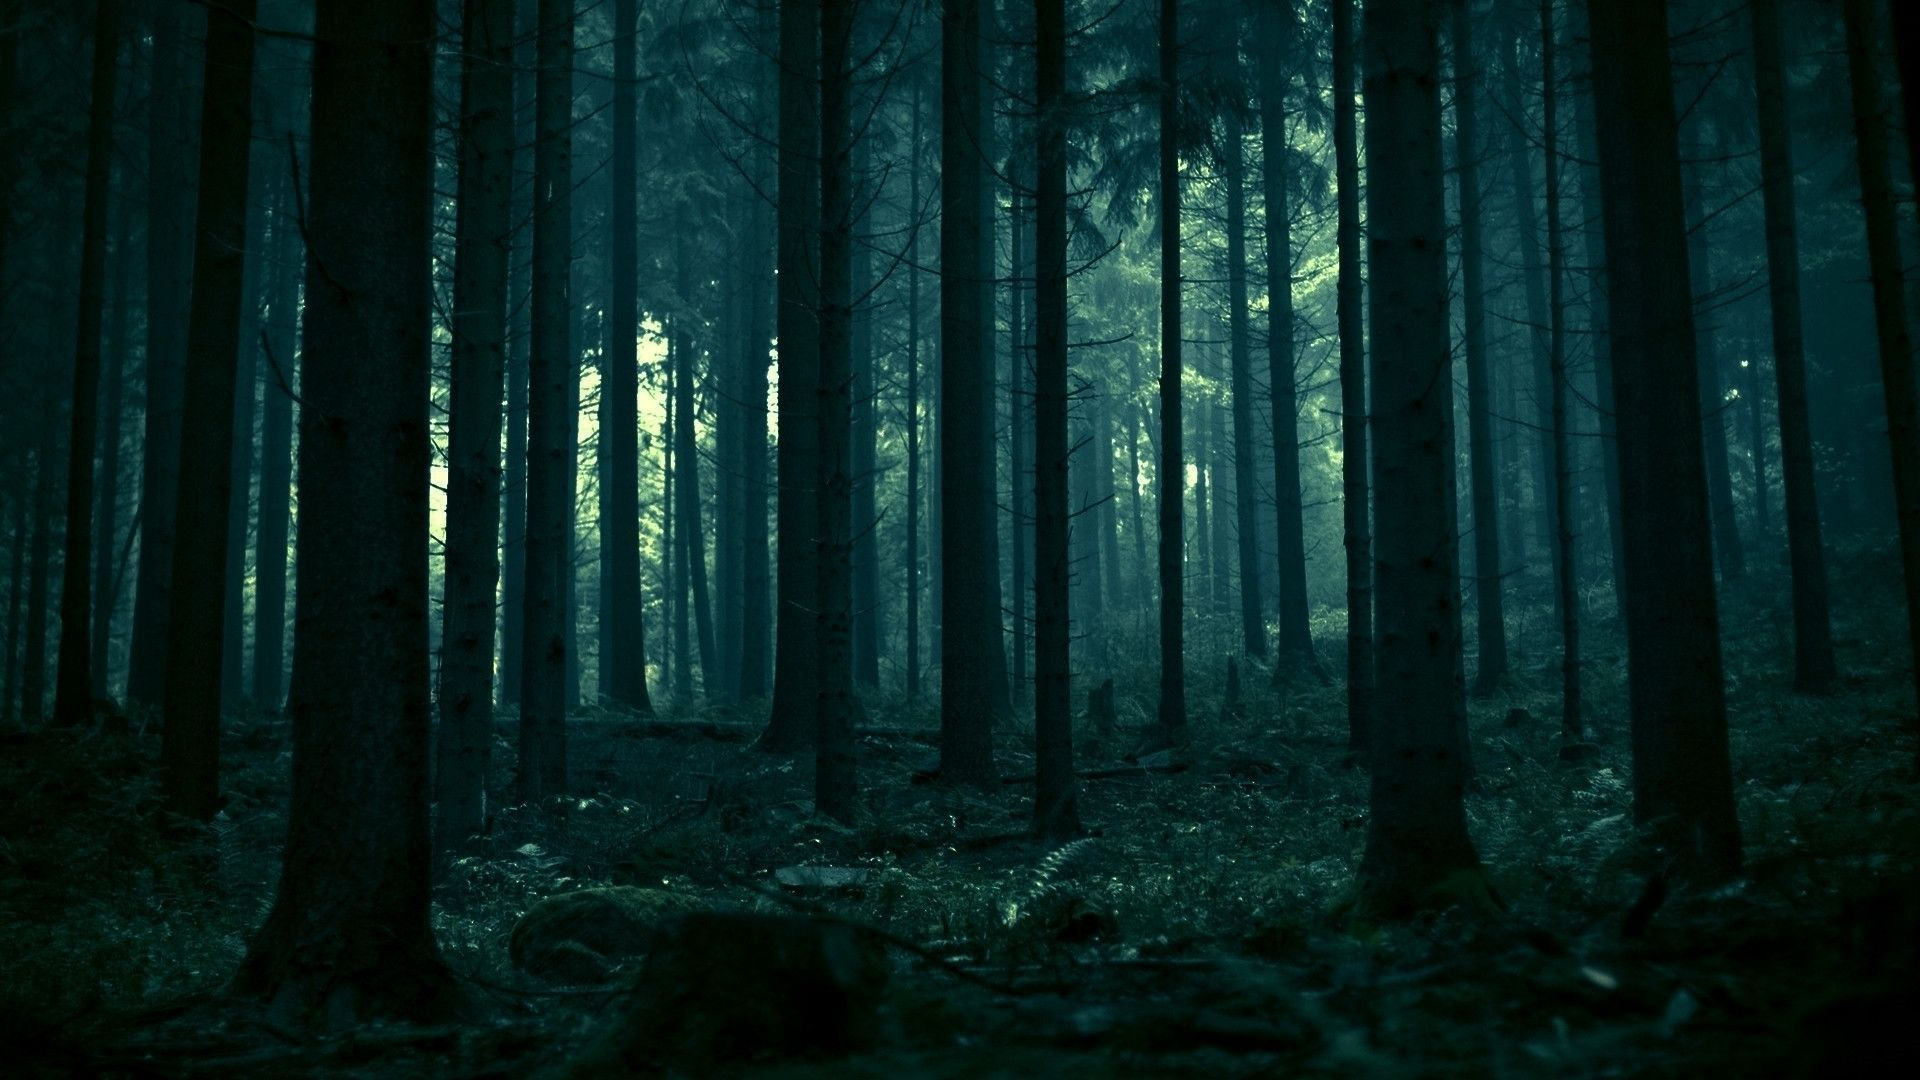
\includegraphics[max width=\textwidth]{../Pictures/Locations/Hogwarts/Forbidden_Forest_picture.jpg} 
\end{figure}


\begin{wrapfigure}[11]{r}{0.5\linewidth}
\centering
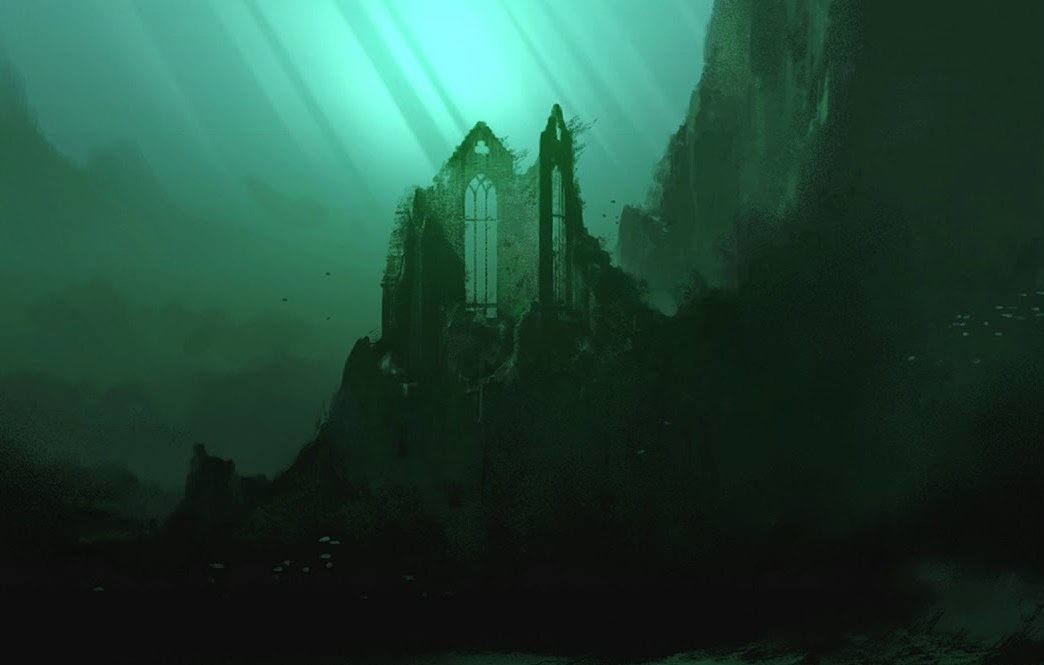
\includegraphics[max width=0.5\textwidth]{../Pictures/Locations/Hogwarts/Black_Lake_picture.jpg} 
\end{wrapfigure}
\paragraph{Black Lake}
A large obscure lake located south of the castle. It is home to various magical sea creatures such as giant squids, mermaids and many more. The seabed temperature is very low, making it a favorable place for algae and other underwater vegetation. Venturing too deep is dangerous since many were attacked and trapped by merpeople.

\begin{wrapfigure}[11]{r}{0.5\linewidth}
\centering
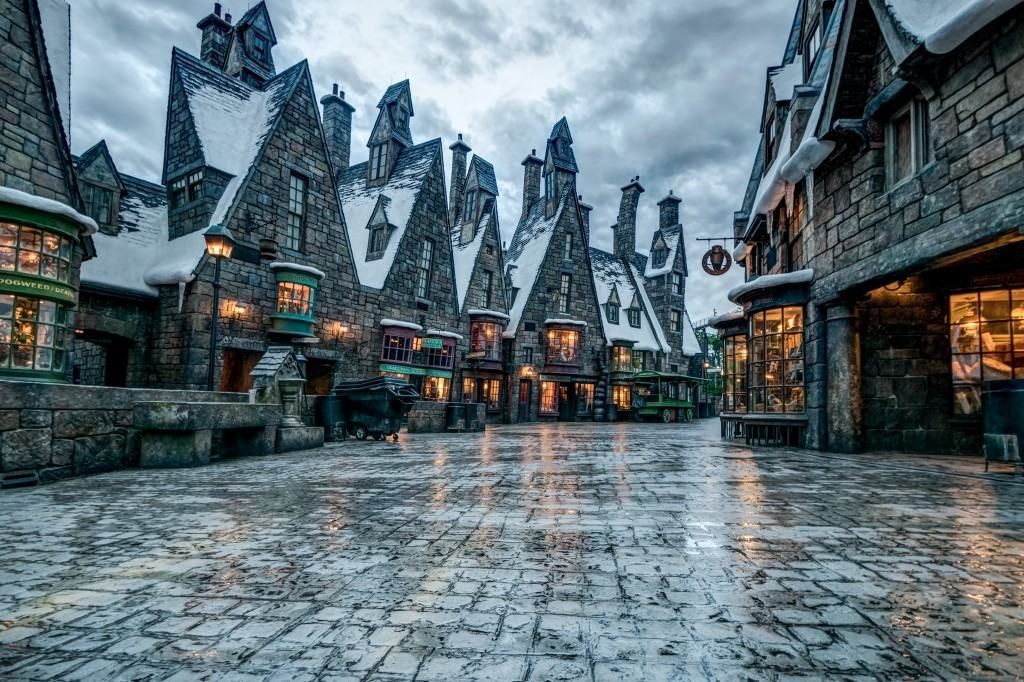
\includegraphics[max width=0.5\textwidth]{../Pictures/Locations/Hogsmeade_picture.jpg} 
\end{wrapfigure}
\paragraph{Hogsmeade}
Picturesque little village near Hogwarts, inhabited only by wizards. Students can usually frequent it during holidays or weekends; they are easily attracted to this village because there are numerous entertainment places, such as pubs, shops. The most famous are The Three Broomsticks or the Zonko's jokes and tricks shop. It is also the terminal station of the Hogwarts Express. 

\begin{wrapfigure}[11]{r}{0.5\linewidth}
\centering
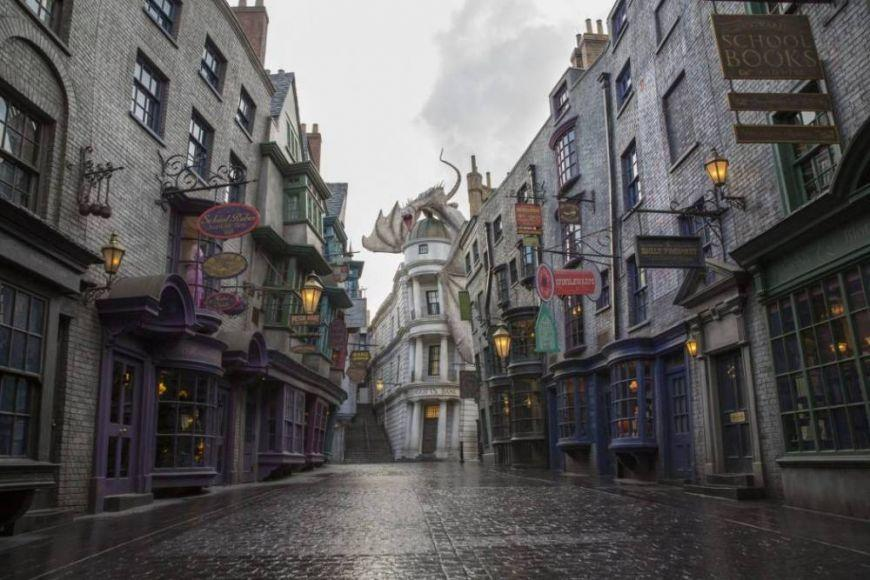
\includegraphics[max width=0.5\textwidth]{../Pictures/Locations/DiagonAlley_picture.jpg} 
\end{wrapfigure}
\paragraph{Diagon Alley}
It's a magical side-street accessible from the muggle city London. To enter Diagon Alley, you need to give a tap on the right bricks of the wall behind Leakey Cauldron, which will move and reveal the entrance to the street. It can also be accessed via Flying Dust or dematerialization. The magic street has various important magical shops, such as Ollivander's Wand store.

\pagebreak
